\title{Автоматизация транспортного предприятия}
\author{Бушкин А. (САПР-1.1н), \\
  Голубев А. (САПР-1.1п), \\
  Чечеткин И. (САПР-1.1п)}
\institute{}
\date{}

\begin{frame}
  \titlepage
\end{frame}

\begin{frame}
%  \small
  Автоматизировать транспортное предприятие, осуществляющее перевозку грузов
  и пассажиров автомобильным транспортом по России. \textbf{Целью}
  автоматизации является снижение стоимости перевозок.
  
  \vspace{5mm}
  \textbf{Задачи:}
    \begin{itemize}
      \item исследование объекта;
      \item выделить слабые стороны рабочего процесса;
      \item выбрать самое подходящее решение проблемы.
    \end{itemize}
\end{frame}

\begin{frame}
  \frametitle{AS IS}
  \begin{center}
    \begin{figure}
      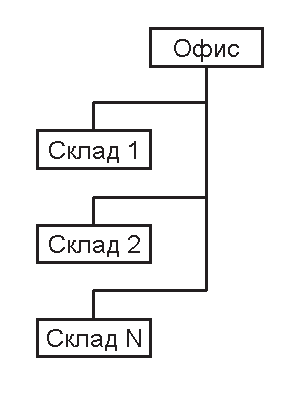
\includegraphics[width=.25\textwidth]{as_is_1}
      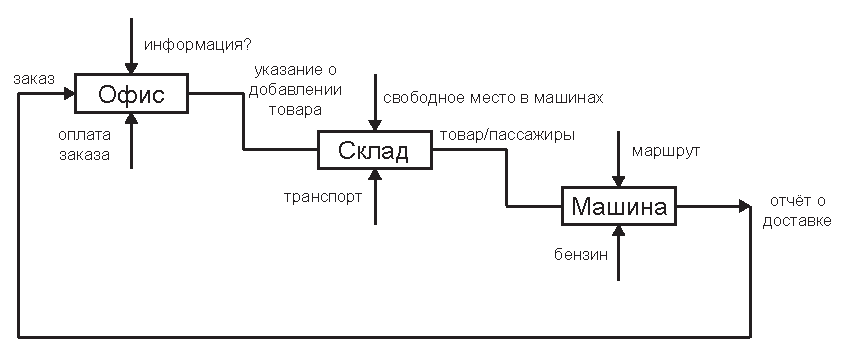
\includegraphics[width=.75\textwidth]{as_is_2}
    \end{figure}
  \end{center}
\end{frame}

\begin{frame}
  \frametitle{Предложения:}
  \begin{enumerate}
    \item автоматическое планирование маршрутов грузовых перевозок с учетом
      загруженности машины как в одну, так и в обратную сторону;
    \item создание списка рейсовых маршрутов как пассажирского, так и
      грузового транспорта;
    \item поддержка срочных частных заказов;
    \item отчетность об отбытии/прибытии в ключевые точки маршрута через БД.
  \end{enumerate}
\end{frame}

\begin{frame}
  \frametitle{TO BE}
  \begin{center}
    \begin{figure}
      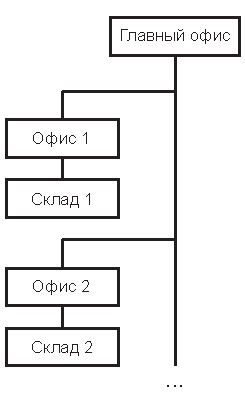
\includegraphics[width=.25\textwidth]{to_be_1}
      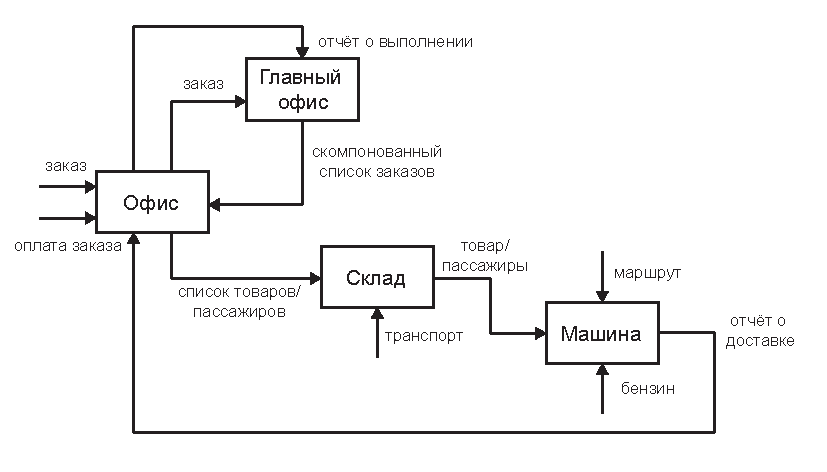
\includegraphics[width=.75\textwidth]{to_be_2}
    \end{figure}
  \end{center}
\end{frame}

\begin{frame}
  \frametitle{Необходимые ресурсы:}
  \begin{enumerate}
    \item система автоматизированного составления маршрута с учетом
      заполненности машины на весь маршрут, сезонности и др. факторов;
    \item система проектирования рейсовых маршрутов;
    \item сервер в главный офис, СУБД, офисное оборудование;
    \item организация сети между компьютерами компании.
  \end{enumerate}
\end{frame}

\begin{frame}
  \frametitle{Затраты на ресурсы:}
  \begin{enumerate}
    \item офисное оборудование: \( \sim\, \)500 тыс.~\rouble;
    \item сервер в главный офис: \( \sim\, \)150 тыс.~\rouble;
    \item разработка системы автоматизированного планирования маршрутов:
      \( \sim\, \)200 тыс.~\rouble;
    \item поддержка пунктов 2 и 3: \( \sim\, \)30 тыс.~\rouble\ в месяц;
    \item закупка стороннего ПО (СУБД и etc): \( \sim\, \)100 тыс.~\rouble.
  \end{enumerate}
\end{frame}

\begin{frame}
  \frametitle{Результат автоматизации:}
  \begin{enumerate}
    \item экономия денежных средств (в долгосрочном периоде) на перевозке
      грузов за счет гибкого планирования маршрутов;
    \item автоматизация в составлении маршрутных листов и сокращение штата
      сотрудников;
    \item децентрализованная работа с клиентами;
    \item готовая система для простой организации новых офисов.
  \end{enumerate}
\end{frame}